% !TeX spellcheck = en_GB
\documentclass[10pt,letterpaper,oneside]{article}
\usepackage{fontspec}
\usepackage{arev}
\usepackage[utf8]{inputenc}
\usepackage[T1]{fontenc}
\usepackage{amsmath}
\usepackage{amsfonts}
\usepackage{amssymb}
\usepackage{graphicx}
\usepackage{csquotes}
\usepackage{booktabs}
\usepackage{multicol}
\usepackage{enumerate}
\usepackage{microtype}
\usepackage[labelfont=bf,font={small}]{caption}
\usepackage{hyperref}
\usepackage{booktabs}
\usepackage{subcaption}
\usepackage{fancyhdr}
\usepackage[svgnames]{xcolor}
\usepackage{mdframed}
\usepackage{multicol}
\usepackage[para]{footmisc}
\usepackage{siunitx}
\usepackage{cleveref}
\usepackage{listings}
\usepackage{cprotect}


\lstset{ % General setup for the package
	language=Python,
	basicstyle=\small\ttfamily,
	tabsize=4,
	columns=fixed,
	showstringspaces=false,
	showtabs=false,
	keepspaces,
	commentstyle=\color{SeaGreen},
	keywordstyle=\bf\ttfamily\color{DarkBlue}
}

\newfontfamily\symbolfont{Symbola}
\usepackage[left=1in,right=1in,top=1in,bottom=1in,marginparwidth=0.3in]{geometry}

\usepackage[sorting=none]{biblatex}
\addbibresource{../bibliography.bib}

\author{Andreas Stöckel\\[0.5cm]Based on lecture notes by\\Chris Eliasmith and Terrence~C.~Stewart}
\newcommand{\baseCodeURL}{https://github.com/astoeckel/syde556-w20/blob/master/lectures}

\fancyhf{}
\fancyhead[L]{SYDE 556/750 Lecture Notes}
\fancyhead[R]{Andreas Stöckel}
\fancyfoot[C]{\thepage}
\pagestyle{fancy}

\setlength{\parindent}{0em}
\setlength{\parskip}{0.5em}
\renewcommand{\baselinestretch}{1.25}
\renewcommand{\vec}[1]{{\mathbf{#1}}}
\newcommand{\mat}[1]{{\mathbf{#1}}}
\newcommand{\T}{\ensuremath{\mathrm{T}}}
\renewcommand{\epsilon}{\varepsilon}
\renewcommand{\phi}{\varphi}

\makeatletter
\newcommand{\superimpose}[2]{%
	{\ooalign{{#1}\hidewidth\cr{#2}\hidewidth\cr}}}
\makeatother
\newcommand{\SolidCircle}[2]{\superimpose{\color{#1}\symbolfont ⬤}{\textbf{\color{white}#2}}\hspace{1em}}
\newcommand{\OPlus}{\SolidCircle{DarkGreen}{\kern0.75pt+}}
\newcommand{\OMeh}{\SolidCircle{DarkOrange}{~}}
\newcommand{\OMinus}{\SolidCircle{DarkRed}{\kern2.25pt--}}

\newcommand{\YouTube}[2][Video]{\href{https://youtu.be/#2}{{\symbolfont 📺}~{#1}}%
%\footnote{\url{https://youtu.be/#2}}%
}

\newcommand{\CodeLink}[2][Code]{\href{\baseCodeURL/#2}{{\symbolfont ⌨}~\emph{#1}}}

\newcommand{\MakeTitle}[1]{
\maketitle
\begin{center}
	
\includegraphics[width=0.5\textwidth]{../assets/uwlogo.pdf}\\[1cm]
	{#1}\
\end{center}

\vfill

\thispagestyle{empty}
\setcounter{page}{0}
\newpage

\pagenumbering{roman}
\setcounter{tocdepth}{2}
\tableofcontents
\newpage

\setcounter{page}{0}
\pagenumbering{arabic}}

\reversemarginpar


\newcommand{\ColorBox}[3]{%
	\marginpar{%
		\huge\raisebox{-3ex}{\symbolfont{#1}}%
	}%
	\begin{mdframed}[hidealllines=true,backgroundcolor=#2,innertopmargin=0.25cm,innerbottommargin=0.25cm]%
		{#3}
	\end{mdframed}}

\newcommand{\Note}[1]{\ColorBox{📌}{WhiteSmoke}{\textbf{Note:} #1}}
\newcommand{\Example}[1]{\ColorBox{💡}{WhiteSmoke}{\textbf{Example:} #1}}
\newcommand{\Aside}[1]{\ColorBox{🌟}{WhiteSmoke}{\emph{Aside:} #1}}
\newcommand{\Python}[1]{\ColorBox{🐍}{WhiteSmoke}{#1}}
\newcommand{\Notation}[1]{\ColorBox{\huge$\Sigma$}{WhiteSmoke}{\textbf{Notaton:} #1}}

\newcommand{\ConstructionSite}{\hrulefill {\symbolfont 🚧} UNDER CONSTRUCTION {\symbolfont 🚧} \hrulefill}

\newenvironment{ImportantEqn}[1]{\mdframed\raggedleft\emph{({#1})}\align}{\endalign\endmdframed}

\date{January 23 \& 28, 2020}
\title{SYDE 556/750 \\ Simulating Neurobiological Systems \\ Lecture 4: Temporal Representation}


\begin{document}

\MakeTitle{\textbf{Accompanying Readings: Chapter 4 of Neural Engineering}}

\section{Introduction}

\Note{We set out to build a theory of what \enquote{the neural code} may be. In Lecture 2 we discussed individual neuron models, and roughly modelled their behaviour in terms of a rate approximation $G[J]$. We continued in Lecture 3 to think about \enquote{representation} in groups of neurons, i.e.,~what the \emph{activity} of individual neurons represents in terms of (external) stimuli. While this brings us closer to a theory of the \enquote{neural code}, one important notion has been missing so far: time.}

We discussed how neural populations could be modelled as representing vectorial quantities. In this process, we assumed that each neuron in the population computes a spike rate $G[J]$ in spikes per second, given an input current $J$. As we saw when we were discussing the LIF neuron model, this is not the case in biology. Neurons are dynamical systems that take a stimulus over time and output a sequence of action potentials or \emph{spikes}.

The output of a biologically plausible neuron model is also so called a \emph{spike train}. Given an input current over time, the $i$-th neuron in a neural population produces a series of output spikes at time points $t^1_i, t^2_i, \ldots$. We model a spike train as a continuous function over time by superimposing a set of Dirac-$\delta$ functions
\begin{align*}
	a_i(t) &= \sum_{k = 1}^\infty \delta\big(t - t^k_i\big) \,.
\end{align*}

\Note{As detailed in the notes for Lecture 2, the Dirac-$\delta$ function is defined as the function $\delta(t)$ that is zero for all points $t \neq 0$, but has an integral of one.}

As before, our goal is to decode (\enquote{read out}) the value represented in the neural population. However, in contrast to what we did before, we would like to decode the value represented in the population at \emph{any time} $t$. We will solve this problem in three parts: first, we explore what happens if we use exactly the same technique we used before on the spike trains produced by a neural population. Then, we try to remove noise in the estimate by computing an optimal filter. Lastly, we consider what the biological correlate of such a filter could be.

\section{Solving for a Spike Train Decoder}

Our first attempt at decoding a neural representation is similar to what we did before -- we will gather a bunch of training data, consisting of a time-series of neural activity $\vec a(t)$ and a represented value $\vec x(t)$. We arrange discrete samples of these activities in matrices $\mat A$ and $\mat X$ and compute a decoder $\mat D$. Then, we can decode the represented value according to the decoding equation $\hat{\vec x}(t) = \mat D \vec a(t)$.


\subsection{Discretizing Spike Trains}

In the previous lecture, we discussed computing a decoder $\mat D$ by choosing a random set of $N$ samples $\big\{ \vec x_1, \ldots, \vec x_N \big\} \subset \mathbb{X}$, forming a matrix $\mat X \in \mathbb{R}^{d \times N}$, as well as recording the associated nonnegative population activities $\big\{ \vec a(\vec x_1), \ldots, \vec a(\vec x_N) \big\} \subset \big(\mathbb{R}^{+} \big)^n$, forming a matrix $\mat A \in \big(\mathbb{R}^{+}\big)^{n \times N}$.

Now, the question is how to gather such training data in the time-continuous case. One procedure that could accomplish this is to generate a random, bandlimited signal $\vec x(t)$, feeding this signal into the neuron population, and recording the neural activities. In other words, for each neuron $i$ in the population, we have the encoding equation
\begin{align*}
J_i(t) &= \alpha_i \langle \vec e_i, \vec x(t) \rangle + J^\mathrm{bias}_i \,, \\
a_i(t) &= \sum_{k=1}^\infty \delta\big(t - t^k_i\big) \,,
\end{align*}
where $t^k_i$ is the time of the $i$-th spike produced by our neuron model for an input current $J_i(t)$. In case we chose the LIF neuron model, we would for example use $J_i(t)$ as an input in the following sub-threshold differential equation
\begin{align*}
\frac{\mathrm{d}}{\mathrm{d}t} v_i(t) &= -\frac{1}{\tau_\mathrm{RC}} \big( v_i(t) - J_i(t) \big)
\big) \,, \quad &\text{if } v_i(t) &< 1\,,
\end{align*}
with the appropriate super-threshold behaviour following spike production -- whenever $v_i(t)$ reaches the threshold potential $v_\mathrm{th} = 1$ we clamp the membrane potential to the reset potential $v_\mathrm{reset} = 0$ for $\tau_\mathrm{ref}$ seconds
\begin{align*}
v(t) &\gets 0 \,, &\text{if } t &> t_i^k\mathrm{th} \text{ and } t \geq t_i^k + \tau_\mathrm{ref} \,, \text{for all spike times } t_i^k \,.
\end{align*}

To summarize, we have two time-continuous functions: $\vec x(t)$, our randomly created input function, and $\vec a(t)$, the spike trains produced by our neurons for the given represented values.

So, how do we assemble our matrices $\mat X$ and $\mat A$, which need to be constructed out of $N$ discrete values? Well, we simply discretise our function into short time-slices of width $\Delta t$, starting at a time zero, and stopping at a time~$T$. We then have $N = \lfloor T / \Delta t \rfloor$ time slices -- each of these time slices can be interpreted as one of $N$ samples for our matrix.

\Note{\emph{Discrete Dirac-$\delta$.} While generating a discrete input function $\vec x(t)$ may be fairly straight forward (we can use the Discrete Fourier Transformation (DFT) to generate a bandlimited input function, see below), discretising the spike trains $\vec a(t)$ might be a little unintuitive, since each $a_i(t)$ is a sum of Dirac-$\delta$ functions. Luckily, this can be easily resolved by recalling the two important properties of the Dirac-$\delta$ listed above: being zero at all except for one point, and the integral being one. In the discrete case this means that the Dirac-$\delta$ is zero for all sample points except for one sample point which we have to set to $\Delta t^{-1}$ to get an area-under-the-curve of one when we discretise the integral. Assuming we have a spike at time $t'$ with $0 < t' < T$, we get
\begin{align*}
	\int_{0}^T \delta(t - t') \,\mathrm{d}t &= \sum_{i = 1}^N f_i \Delta t = \frac{\Delta t}{\Delta t} = 1 \,, &\text{where } f_i &=
	\begin{cases}
		\frac{1}{\Delta t} & \text{if } i \neq \left\lfloor\frac{t'}{\Delta t}\right\rfloor \,,\\
		0 & \text{otherwise} \,, \\
	\end{cases}
\end{align*}
where $f_i$ are the discrete samples of the function.
}

\subsection{Computing Decoders}

\begin{figure}[p]
	\begin{subfigure}[b]{0.4\textwidth}
		\centering
		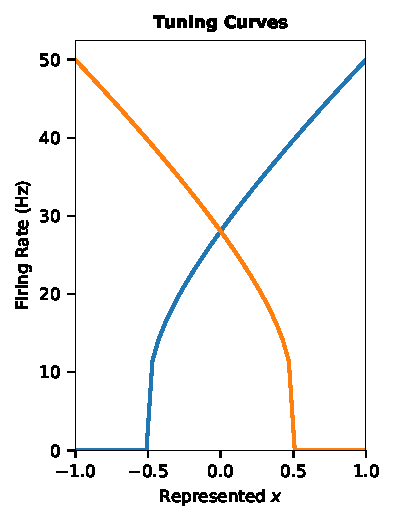
\includegraphics{media/two_neurons_tuning_curves.pdf}
		\caption{Population Tuning}
	\end{subfigure}
	\begin{subfigure}[b]{0.6\textwidth}
		\centering
		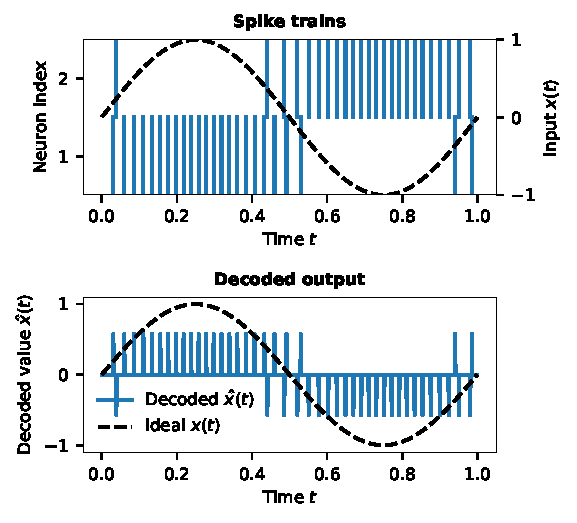
\includegraphics{media/two_neurons_spike_train.pdf}
		\caption{Spike Trains and Decoding}
	\end{subfigure}
	\caption{\textbf{(a)} Neural population tuning curves for two neuron. \textbf{(b)} Recorded spike trains for a sine-wave input (\emph{top}) and decoded output (\emph{bottom}). Time step of $\Delta t = \SI{1}{\milli\second}$. \CodeLink{lecture_04/media/code/time_continuous_decoding_experiment.ipynb}}
	\label{fig:two_neurons}
\end{figure}

\begin{figure}[p]
	\begin{subfigure}[b]{0.4\textwidth}
		\centering
		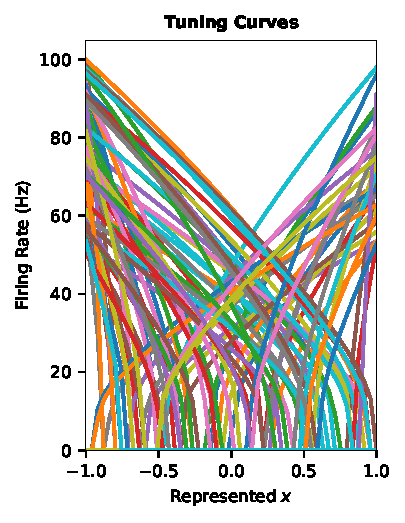
\includegraphics{media/hundred_neurons_tuning_curves.pdf}
		\caption{Population Tuning}
	\end{subfigure}
	\begin{subfigure}[b]{0.6\textwidth}
		\centering
		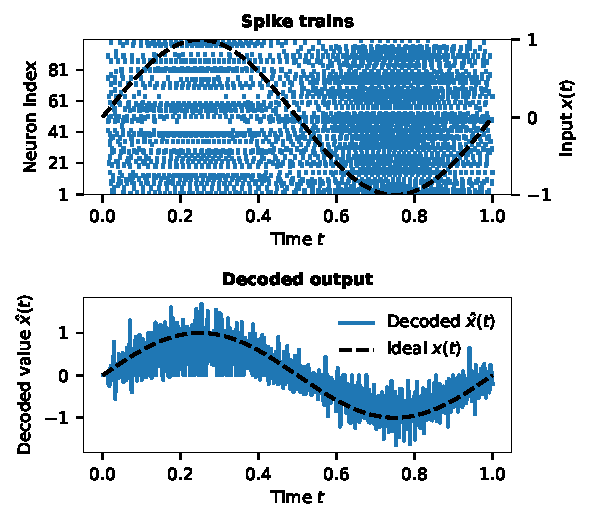
\includegraphics{media/hundred_neurons_spike_train.pdf}
		\caption{Spike Trains and Decoding}
	\end{subfigure}
	\caption{\textbf{(a)} Neural population tuning curves for one hundred neurons. \textbf{(b)} Recorded spike trains for a sine-wave input (\emph{top}) and decoded output (\emph{bottom}).  Time step of $\Delta t = \SI{1}{\milli\second}$. \CodeLink{lecture_04/media/code/time_continuous_decoding_experiment.ipynb}}
	\label{fig:hundred_neurons}
\end{figure}

Given a discretised version of our input function $\vec x(t)$ and the recorded population spike trains $\vec a(t)$, we can finally construct matrices $\mat X$ and $\mat A$ and use these to compute a set of decoders $\mat D$ according to the least-squares solution we discussed in the last lecture
\begin{align*}
	\mat D^\T &= (\mat A \mat A^\T)^{-1} \mat A^\T \mat X \,.
\end{align*}
Note that is it not necessary to use the regularised version of this equation. As we discussed last lecture, regularisation is not necessary if we have a large number of noisy samples -- which is exactly what we have in this case. For example, if we record neural activities for a few neurons over $T = \SI{10}{\second}$ at a time step of $\Delta t = \SI{1}{\milli\second}$ we already have \num{10000} samples for each neuron.

\Note{\emph{Interpretation of the decoder computation equation.} If we analyse the above equation more thoroughly ({\symbolfont 🚧} \emph{I will insert this here at a later point}), we see that we are implicitly approximating the average firing rate for each neuron, giving a certain input $\vec x$.
	
In a sense, we are computing the rate approximation $G[J]$ of the individual neurons \enquote{on the fly}. This has the consequence that our decoders $\mat D$ computed using the rate approximation $G[J]$ should still work in a spiking context. However, one advantage of this way of computing decoders is that it also works for more complicated neuron models for which we cannot easily compute a rate approximation $G[J]$.}

\paragraph{Example: Decoding from two neurons}
\Cref{fig:two_neurons} shows an example of what we have discussed above. In this particular case, we choose neural parameters $e_i$, $\alpha_i$, $J^\mathrm{bias}_i$ such that we have one neuron approximately covering the positive space of represented values, and another neuron covering the negative space of represented values. The decoder $\vec d$ for these two neurons is approximately
\begin{align*}
	\vec d = \begin{pmatrix} 0.5 \Delta t, & -0.5 \Delta t \end{pmatrix} \,.
\end{align*}
Whenever we receive a spike from the first neuron (each spike modelled as a discrete Dirac-pulse of height $1/\Delta t$) we decode out $0.5$, whenever we receive a spike from the second neuron we decode out $-0.5$. We do not have any information \enquote{in between spikes}.

\paragraph{Example: Decoding from one hundred neurons}
If we increase the number of neurons, the chance of multiple neurons spiking in the same timestep increases. In this case, our decoded output actually starts to look more like what we would expect (\cref{fig:hundred_neurons}) -- in particular, since is a smaller change of being \enquote{in between spikes}, the decoded output does not constantly return to zero. Unfortunately, this is solely an artefact of discretisation. As we decrease our timestep $\Delta t$, it gets less and less likely for two neurons to be spiking in exactly the same timestep.


\section{Temporal Filtering}

% TODO

\paragraph{Filtering}
\begin{itemize}
	\item Problem: No data when there are no spikes
	\item Idea: Filter the output spikes with a filter $h$
	\begin{align*}
		\hat{\vec x}(t) &= D (\vec a \ast h)(t)
	\end{align*}
	\item Scalar case:
	\begin{align*}
		\hat x(t) &= \sum_{i = 1}^n d_i (a_i \ast h)(t)
	\end{align*}
	\item Convolution operator:
	\begin{align*}
		\big( f \ast g \big)(t) \overset{\text{def}}= \int_{-\infty}^{\infty} f(t - \tau) g(\tau)
	\end{align*}
	\item Which filter to chose? Gaussian filter ($\Rightarrow$ slides)
\end{itemize}

\paragraph{Random signals}

(See slides)

\paragraph{Optimal filter}

\begin{itemize}
	\item Special case: two neurons, same $\alpha$ and $J^{bias}$ but different $e$ ($-1$ and $+1$)
	\item Neurons are symmetric opposites, we can assume $d_1 = -d_2$
	\item Hence 
	\begin{align*}
		\hat x(t)
			&= \big(a_1 d_1 + a_2 d_2) \ast h \big)(t)\\
			&=  d_1 \big((a_1 - a_2) \ast h \big)(t)
	\end{align*}
	\item Fold the constant into $h$:
	\begin{align*}
		\hat x(t) &= \big((a_1 - a_2) \ast h \big)(t) \\
				  &= \big(\underbrace{r}_{\text{response}} \ast h \big)(t)
	\end{align*}
	\item \textbf{Goal:} Find filter $h$ that minimizes error:
	\begin{align*}
		E = \int_{-\infty}^\infty \left( x(t) - \big(r \ast h\big)(t) \right)^2 \,\mathrm{d}t
	\end{align*}
	\item \textbf{Problem:} Convolution is annoying
	\item \textbf{Idea:} Fourier domain, convolution turns into multiplication
	\begin{align*}
		\hat{X}(\omega) = R(\omega)H(\omega)
	\end{align*}
	\item Find $H$ that minimizes error
	\begin{align*}
		E = \int_{-\infty}^{\infty} \big( X(\omega) - R(\omega) H(\omega) \big)^2 \,\mathrm{d}\omega
	\end{align*}
	\item Derivative, set to zero:
	\begin{align*}
		H(\omega) = {{X(\omega) \overline{R}(\omega)} \over {|R(\omega)|^2}} \,, \text{ where } \overline{z} = \overline{x + iy} = x - iy \text{ complex conjugate}
	\end{align*}
	Optimal filter for a signal $X$ and a response $R$. Optimize over a large range of values.
	\item Improvement: We know that we want to reject high frequencies. Add some windowing:
	\begin{align*}
		H(\omega)= {{(X(\omega)R^*(\omega)) \ast W(\omega)} \over {|R(\omega)|^2 \ast W(\omega)}} \,,
	\end{align*}
	where $W(\omega)$ is a Gaussian window function.
\end{itemize}




%\subsection{Exploring the Optimal Filter}

%\subsection{Discussion}

%\hrulefill {\symbolfont 🚧} To be finished {\symbolfont 🚧} \hrulefill

%\section{Using the Synapse as a Filter}

%\subsection{Synaptic Filters}

%\subsection{Exploring Synaptic Filters}

\printbibliography

\end{document}
